\documentclass[12pt]{article}
\usepackage[spanish, english, es-tabla]{babel}
\usepackage[utf8]{inputenc}
\usepackage{amsmath,amssymb}
\usepackage{graphicx}

\usepackage{array}

\usepackage[dvipsnames]{xcolor}

\usepackage{hyperref}
\usepackage{subcaption}
\usepackage[left = 2cm, right = 2cm, bottom = 2cm, top = 3cm]{geometry}

\hypersetup{
	colorlinks=true,
	linkcolor=black,
	%filecolor=magenta,      
	urlcolor=cyan,
}

\hypersetup{
	pdftitle= {Diseño y automatización de sistema de alimentación para animales a través de la tecnología LoRa},
	pdfauthor = {Lucía Francoso Fernández},
	pdfsubject = {Electrónica y comunicaciones móviles},
	pdfkeywords = {Arduino, LoRa, automatización, LoRaWAN, punto a punto, OpenSource}
}

\begin{document}
	\selectlanguage{spanish}

	\title{Diseño y automatización de sistema de alimentación para animales a través de la tecnología LoRa}
	\author{Lucía Francoso Fernández}
	\date{Marzo 2021}
	
	\maketitle
	\pagebreak
	
	\tableofcontents
	
	\pagebreak

	\listoffigures
	\addcontentsline{toc}{section}{Índice de figuras}

	\listoftables
	\addcontentsline{toc}{section}{Índice de tablas}
	
	\section[Introducción]{Introducción} %corchetes, marcapaginas, llaves, texto
	
	Tras finalizar los estudios de grado en ingeniería en sistemas de telecomunicaciones, se requiere como último paso para la obtención del título la elaboración del \textit{Trabajo Fin de Grado} (TFG). 
	El TFG como tal tiene unos objetivos claros, los cuales son demostrar que se han adquirido las competencias básicas intrínsecas al grado, y que el alumno es capaz de seguir aprendiendo a partir de los conocimientos ya obtenidos, innovar, desenvolverse ante un problema determinado y, en resumen, saber llevar a cabo una investigación o proyecto que tenga como objetivo la resolución de dicho problema. \\
	
	\noindent En este documento, se recoge el proyecto realizado como TFG,  el cual va en línea con la filosofía y objetivos del \textit{Trabajo Fin de Grado} en sí mismo. Se detallará el proceso de creación de un sistema de alimentación para animales automatizado, donde se monitorizan de manera remota el estado de los tanques de reserva de agua y pienso. Así, se pretende exponer el conjunto de elementos hardware y software que serán necesarios para monitorizar, automatizar y acceder a ciertos datos de forma remota empleando, principalmente, Arduino y LoRa.\\
	
	
	\subsection[Contexto y justificación del trabajo]{Contexto y justificación del trabajo}

	\noindent Este proyecto ha sido concebido con el objetivo principal de ayudar a la preservación de la vida animal, ante el aumento de especies en extinción, sobretodo en lo que llevamos de siglo \footnote{\href{https://www.nationalgeographic.com.es/naturaleza/grandes-reportajes/animales-peligro-extincion_12536}{National Geographic} , \href{https://www.bbc.com/mundo/noticias-54036796}{BBC}, \href{https://www.worldwildlife.org/descubre-wwf/historias/que-significa-especie-en-peligro-de-extincion}{WWF}, \href{https://www.fundacionaquae.org/causas-perdida-biodiversidad/}{Fundación AQUAE}}, y ante el hecho de que miles de animales domésticos siguen siendo abandonados al año en España \footnotemark. \\
	
	%Fundación Affinity, 20 minutos, La Razón, RTVE
	\footnotetext{\href{https://www.fundacion-affinity.org/observatorio/infografia-el-nunca-lo-haria-estudio-de-abandono-y-adopcion-2020}{Fundación Affinity}, \href{https://www.20minutos.es/noticia/4318383/0/el-abandono-animal-en-espana-aumenta-un-25-en-las-ultimas-semanas/}{20 minutos}, \href{https://www.larazon.es/medio-ambiente/20201118/qxv6yuokargfbnjvknn6bhm4ze.html}{La Razón}, \href{https://www.rtve.es/noticias/20200608/abandonos-animales-domesticos-se-han-disparado-espana-durante-meses-confinamiento/2015761.shtml}{RTVE}}

	\noindent Es por ello que se requiere de ayuda activa para paliar estos problemas. Las tareas de carácter solidario, en bastantes casos, no siempre cuentan con suficientes voluntarios; además, siendo un problema tan extendido y avanzado, el número de acciones que hay que llevar a cabo para aliviarlo es alto para un número limitado de voluntarios, los cuales deben incrementar considerablemente el tiempo que pasan realizando este tipo de tareas. 
	Tanto si se trata de un refugio de animales domésticos abandonados, como de reservas naturales donde se intenta repoblar una especie, los animales dependen enteramente del trabajo de los voluntarios. Así pues, es de vital importancia la optimización de las tareas de voluntariado, su automatización e, incluso, control remoto, mediante la creación de herramientas que ayuden a reducir el tiempo que se destina a tareas rutinarias para poder utilizar ese tiempo a otras tareas (de rescate, o de financiación para el mantenimiento de las instalaciones y de los propios animales, por ejemplo). \\
	
	\noindent Con el objetivo en mente de ayudar a la preservación de la fauna (y con ello, de la vida de los ecosistemas terrestres), evitando la extinción de especies y el abandono animal, se ha concebido y desarrollado este proyecto teniendo en cuenta los diferentes casos de uso (emplazamientos donde se podrá instalar el sistema, características del entorno), mejor adaptación a ellos, relación entre buenas prestaciones y bajo consumo, precio total del producto, o facilidad de uso por parte de un usuario medio. Es por ello que desde el principio se propone una serie de actuaciones a realizar, acorde a lo anteriormente mencionado, tales como:
	
	\begin{itemize}
		\item El diseño del sistema de alimentación será tal que el producto final pueda ser instalado no sólo en hogares, sino en sitios remotos, donde el acceso a recursos tales como la electricidad o Internet son escasos o inexistentes. Así pues, el dispositivo utilizará energía solar y baterías recargables, comunicación de bajo consumo y largo alcance y modo de ahorro de energía. 
		\item El dispositivo final no será pesado ni voluminoso, facilitando así tanto su transporte como su manejo. No dejará al alcance del animal electrónica, de manera que evitaremos que los animales estén en contacto con ella y posibles problemas de humedad presente en el entorno; se usarán protecciones adecuadas a la calidad de los componentes del dispositivo.
		\item El dispositivo contará con una pantalla OLED que permitirá ver a la persona que esté físicamente delante de él si funciona correctamente. También se permitirá el acceso a datos a personas interesadas que quieran consultarlos de manera remota.

	\end{itemize}

	
	\subsubsection[Ejemplo de caso de aplicación]{Ejemplo de caso de aplicación}
	
	Un ejemplo de caso de aplicación sería el entorno donde se desea situar uno de estos dispositivos para validar su funcionamiento, que en este caso se trata del refugio perteneciente a la protectora Patitas Unidas Los Alcázares, situado en el término municipal de Torre Pacheco (Murcia).
	La elección de esta ubicación se fundamenta en una serie de razones:
	
	\begin{itemize}
		\item Al ser voluntaria para esta protectora, conozco bien sus necesidades, es decir, qué puede ser de utilidad para la protectora en el refugio y qué soluciones se han probado para determinados problemas que han ido surgiendo; además, conozco bajo qué condiciones climáticas es vulnerable y qué necesidades esporádicas emergen bajo dichas condiciones. Teniendo en cuenta la zona geográfica donde se ubica (Murcia), y los años de experiencia en el refugio, se ha detectado una problemática que se manifiesta durante  periodos continuados de lluvias (lluvias torrenciales, DANA, gota fría), la cual consiste en la inundación de las zonas colindantes al refugio, inclusive carreteras de acceso, lo que impide llegar a él (cierre de carreteras, niveles altos de riesgo por precipitación, o el simple hecho de contar con grandes volúmenes de agua en la carretera que impiden la circulación segura por la vía). De
		\item Se trata de un entorno sin electricidad y sin internet. Desarrollar un proyecto y probarlo en este tipo de entorno nos ayudará a la hora de extrapolarlo a otros emplazamientos donde la ausencia de este tipo de recursos supone también una limitación y un aspecto a tener en cuenta para definir y desarrollar el proyecto en sí mismo.
		\item Se puede intentar establecer un enlace punto a punto, ya que se puede dejar fijo un equipo transmitiendo o recibiendo que, además, se conecte a internet (ya que es un recurso disponible) para subir los datos que reciba del otro extremo. Un equipo estará presente en el refugio y el otro en una casa con internet y electricidad; esto significa que al menos este extremo será más controlable, y será este extremo el que subirá datos a la nube. Nos tendremos que preocupar más del otro extremo, donde no tendremos electricidad ni internet y donde situaremos los sensores que recogerán datos y realizarán la automatización.
	\end{itemize}
	
	\subsection[Objetivos del trabajo]{Objetivos del trabajo}
	
	El objetivo fundamental del presente trabajo es el diseño de un sistema de alimentación para animales que permita la monitorización de los niveles de agua y pienso que se encuentran en depósitos de reserva, los cuales rellenan un bebedero y un comedero, respectivamente.  Con ello, se pretende automatizar el proceso de alimentación de animales, además del uso de la tecnología LoRa para tener acceso al estado del sistema de forma remota. Así pues, los objetivos concretos son:
	
	\begin{itemize}
		\item Realizar una aproximación a la tecnología LoRa.
		\item Diseñar el sistema de alimentación para animales.
		\item Realizar tanto simulaciones para el enlace LoRa que se creará entre transmisor y receptor, como cálculos teóricos que determinen si el enlace es posible.
		\item Construir el prototipo y probarlo en entorno controlado y, posteriormente, en entorno real.
		\item Crear una plataforma de representación de datos.
	\end{itemize}
	
	\subsection[Enfoque y método seguido]{Enfoque y método seguido}
	\subsection[Planificación del trabajo]{Planificación del trabajo}
	\subsubsection[Alcance]{Alcance}
	\subsubsection[Hitos]{Hitos}	
	\subsubsection[Calendario de trabajo]{Calendario de trabajo}
	\subsubsection[Tareas y diagrama de Gantt]{Tareas y diagrama de Gantt}
	\subsubsection[Riesgos e incidencias]{Riesgos e incidencias}
	\subsubsection[Recursos]{Recursos}
	\subsection[Breve sumario de productos obtenidos]{Breve sumario de productos obtenidos}
	\subsection[Breve descripción de los capítulos restantes de la memoria]{Breve descripción de los capítulos restantes de la memoria}
	
	\pagebreak
	

	\section[Estado del arte]{Estado del arte}  
	
	\noindent En este capítulo se va a exponer un análisis del estado del arte relativo al proyecto (tecnologías y técnicas necesarias para el diseño del sistema planteado). Este análisis se centra en la situación actual en tanto a  la automatización del proceso de alimentación de animales, técnicas, sistemas y proyectos similares y conceptos introductorios a Arduino y LoRa, fundamentales para poder materializar este proyecto.
	
	\subsection[Contexto actual]{Contexto actual}
	
		\noindent Existen muchos proyectos Open Source relacionados con la alimentación automática o semiautomática de animales domésticos, principalmente gatos y perros. Sin embargo, no existen proyectos que usen LoRa como tecnología radio, sino que emplean la red local WiFi del hogar donde se sitúe el dispositivo de alimentación.
	
	\noindent A pesar de ello, se ha visualizado este tipo de proyectos y tenido en cuenta para el desarrollo del prototipo en tanto a apariencia externa, comodidad de uso, eficiencia de los componentes, o, incluso, opciones para mover el pienso desde la reserva hasta el comedero del animal, o el agua desde la reserva hasta el bebedero.
	
	\subsection[Trabajos relacionados]{Trabajos relacionados}
	

	
	\subsection[Resumen del capítulo]{Resumen del capítulo}
	
	\pagebreak
	
	\section[Diseño del sistema]{Diseño del sistema}
	
	\noindent A lo largo de este capítulo se procede a desglosar el diseño del sistema, exponiendo las tecnologías y los dispositivos que se van a emplear tanto en monitorización como en comunicaciones. Por tanto, tras realizar una pequeña introducción de las tecnologías necesarias en el diseño, se procede empleando una metodología en cascada que vaya presentando a cada paso los subsistemas finalizados y completamente operativos.
	
	\subsection[Funcionalidades a cubrir]{Funcionalidades a cubrir: identificación}
	
	\noindent Teniendo claros los objetivos que se persiguen con este proyecto, el siguiente paso es definir las funcionalidades que ofrecería el sistema global que se pretende crear, ya que a partir de esta definición podremos empezar a deducir y establecer qué componentes son necesarios para llevar a cabo dichas funcionalidades. \\
	
	\noindent Definimos 3 funcionalidades: \\
	
	\begin{enumerate}
		\item Alimentación del dispositivo autónoma
		\item Automatización y monitorización (I): bloque microcontrolador
		\item Automatización y monitorización (II): bloque comunicación radio 
		\item Automatización y monitorización (III): bloque comedero (sensores, actuadores)
		\item Automatización y monitorización (IV): bloque bebedero (sensores, actuadores)
		\item Integridad mediante prototipo exterior
	\end{enumerate}
	
	\subsection[Funcionalidades a cubrir]{Funcionalidades a cubrir: desglose y detección de necesidades asociadas}
	

	% Definición funcionalidades: qué debo hacer y qué necesitaría
	% Investigación componentes (*) e integración (programación)
		%(*) Qué se ha usado, desglosado por funcionalidades: bebedero, comedero, alimentación, microcontrolador y radio.
		% Descripción, foto, foto en prototipo protoboard
	% Definición prototipo provisional: opciones que he descartado, QR de que funciona?
	% Diseño PCB
	% Desarrollo BBDD en servidor y app web para ver el estado del sistema de alimentación
	
	\subsection[Tecnologías necesarias]{Tecnologías necesarias: teoría}
	\subsubsection[Entorno Arduino]{Entorno Arduino}
	
	% Intro: qué es Arduino
	
	Arduino es una plataforma de electrónica \textit{open-source} basada en hardware y software fáciles de usar. Las placas Arduino son capaces de leer entradas (como la luz en un sensor, un dedo pulsando un botón) y convertirlas en salidas (activar un motor, apagar o encender un LED); es decir, como usuarios podemos decirle qué hacer a la placa enviándole una serie de instrucciones al microcontrolador de la placa. Para poder hacer esto último, se hace uso del lenguaje de programación de Arduino (basado en \href{http://wiring.org.co/}{\textit{Wiring}}) y el software de Arduino (IDE, basado en \href{https://processing.org/}{\textit{Processing}}). \\
	
	\noindent A lo largo de los años, Arduino ha sido el corazón de miles de proyectos, desde objetos cotidianos hasta complejos instrumentos científicos. Una comunidad mundial de creadores (estudiantes, aficionados, artistas, programadores y profesionales) se ha reunido en torno a esta plataforma de código abierto, sus contribuciones se han sumado a una increíble cantidad de conocimiento accesible que puede ser de gran ayuda tanto para principiantes como para expertos. \\
	
	\noindent  \textbf{\large Origen} \\ 
	
	\noindent Arduino nació en el Ivrea Interaction Design Institute como una herramienta fácil para la creación rápida de prototipos, dirigida a estudiantes sin experiencia en electrónica y programación. Tan pronto como llegó a una comunidad más amplia, la placa Arduino comenzó a cambiar para adaptarse a las nuevas necesidades y desafíos, diferenciando su oferta desde placas simples de 8 bits hasta productos para aplicaciones de IoT, wearable, impresión 3D y entornos integrados. Todas las placas Arduino son completamente de código abierto, lo que permite a los usuarios construirlas de forma independiente y eventualmente adaptarlas a sus necesidades particulares. El software también es de código abierto y está creciendo gracias a las contribuciones de los usuarios de todo el mundo. \\

	
	\noindent \textbf{\large Características} \\
	
	\noindent La principal característica de Arduino es la simplicidad para trabajar con microcontroladores. A raíz de esto, ofrece una serie de ventajas para sus usuarios, como son:
	\begin{itemize}
		\item \textbf{Es de bajo coste}. Las placas de Arduino son relativamente de bajo coste comparadas con las plataformas de otros microcontroladores. La versión más económica de un módulo Arduino puede ser ensamblada a mano, e incluso los módulos Arduino pre-ensamblados cuestan menos de 50 \$.
		\item \textbf{Multiplataforma}. El software de Arduino, Arduino IDE, es capaz de ejecutarse en Macintosh OSX, Windows y Linux. La mayoría de sistemas de microcontroladores están limitados a Windows.
		\item  	\textbf{Entorno de programación simple y claro}. El software de Arduino (IDE) es fácil de usar para principiantes, sin dejar de ser lo suficientemente flexible para usuarios más avanzados.
		\item \textbf{Software Open Source y extensible}. El software Arduino está publicado como un conjunto de herramientas open source, disponible para ser ampliada por otros programadores a través de librerías basadas en el lenguaje C++; las personas que quieran comprender los detalles técnicos pueden dar el salto de Arduino al lenguaje de programación AVR C en el que se basa. Del mismo modo, se puede agregar código AVR-C directamente en los  programas Arduino si así se desea.
		\item \textbf{Hardware Open Source y extensible}. Los planos de las placas Arduino están publicados bajo licencia \textit{Creative Commons}, así pues, diseñadores de circuitos experimentados pueden hacer su propia versión del módulo, extendiéndola y mejorándola. Incluso usuarios sin experiencia pueden crear una versión en protoboard del módulo para entender cómo funciona y ahorrar dinero.
	
	\end{itemize}

	\noindent \textbf{\large Hardware: placas Arduino} \\
	
	\noindent Existen diferentes placas Arduino, cuya elección dependerá del objetivo que persiga nuestro proyecto y de los requerimientos y limitaciones sobre dicho proyecto. \\
	% Electrónica: arduino nano
	
	\noindent \textbf{\large Software: Arduino IDE}
	
	% Programación: arduinoIDE, void loop y setup, define, etc
	
	\subsubsection[LoRa]{LoRa}
	
	\noindent \textbf{Qué es}\\
	
	\noindent El término LoRa proviene de la unión de las palabras \textit{Long} y \textit{Range}, es decir, largo alcance, evidenciando, así, a través de su nombre una de sus principales características. Se trata de la capa física del protocolo \textit{LoRaWAN}; es a través de esta capa que se permite el establecimiento del enlace de comunicación de largo alcance, mientras que LoRaWAN define el protocolo de comunicación y la arquitectura del sistema para la red. \\
	
	\noindent También se trata de una tecnología inalámbrica propiamente dicha que ofrece una transmisión de largo alcance, bajo consumo y segura para aplicaciones IoT y M2M. Se basa en la modulación de espectro ensanchado, la cual presenta características de bajo consumo como la modulación FSK pero puede ser usada para comunicaciones de largo alcance. Puede ser usada para conectar sensores, gateways, máquinas, dispositivos, animales, personas, etc. de manera inalámbrica a la nube.\\
	
	\noindent \textbf{Planes de frecuencia} \\
	
	\noindent La tecnología LoRa opera en diferentes frecuencias dependiendo de la región en la que nos encontremos, por ejemplo: \\
	
	\begin{itemize}
		\item En Norteamérica, opera en la banda de 915 MHz.
		\item En Europa, en la banda de 868 MHz.
		\item En Asia, en la banda de 865 a 867 MHz y en la banda 920 a 923 MHz, aunque es común también la banda 433 MHz.
	\end{itemize}
	
	\noindent Dado que los planes de frecuencia para LoRa varían según la región, inclusive país, es recomendable asegurarse de las regulaciones vigentes en cada país para el uso del espacio radioeléctrico. A modo resumen y como orientación inicial a este asunto, se puede consultar esta \href{https://www.thethingsnetwork.org/docs/lorawan/frequencies-by-country/index.html}{lista de planes de frecuencia para cada país}, elaborada por \textit{The Things Network}. \\
	
	\noindent \textbf{Origen} \\
	
	\noindent La tecnología LoRa fue creada por una compañía francesa llamada \textit{Cycleo}, la cual posteriormente fue adquirida por Semtech en 2012. Semtech fue el miembro fundador de \textit{LoRa Alliance}, que actualmente es el organismo rector de LoRa Technology. LoRa Alliance es una de las alianzas tecnológicas de más rápido crecimiento. Esta asociación sin ánimo de lucro está formada por más de 500 empresas miembro, comprometidas a permitir la implementación a gran escala de redes IoT de amplia cobertura y baja potencia (LPWAN) a través del desarrollo y la promoción del estándar abierto LoRaWAN.\\
	
	\noindent \textbf{Especificaciones en términos generales de la tecnología LoRa}
	
	\begin{itemize}
		\item Órgano rector: LoRa Alliance
		\item Estándar: 801.15.4g
		\item Frecuencia: banda ISM, 868/916 MHz
		\item Alcance: hasta 5 km (urbano) y hasta 15 km (rural)
		\item Datarate: 27 kbps
		\item Modulación: espectro ensanchado basado en la tecnología de modulación FM
		\item Seguridad: CRC de 32 bits
	\end{itemize}
	 
	 %LoRaWAN is a Low Power, Wide Area (LPWA) networking protocol developed by the LoRa Alliance, that wirelessly connects battery operated ‘things’ to the internet in regional, national or global networks, targeting key Internet of Things (IoT) requirements such as bi-directional communication, end-to-end security, mobility and localization services.
	 
	% LoRaWAN uses unlicensed spectrum in the ISM bands to define the communication protocol and system architecture for the network while the LoRa physical layer creates the long-range communication links between remote sensors and gateways connected to the network. This protocol helps in the quick setup of public or private IoT networks anywhere using hardware and software.
	
	\noindent  \textbf{Regulación LoRa en Europa: ERC 70-03} \\
	
	\noindent \href{https://docdb.cept.org/download/25c41779-cd6e/Rec7003e.pdf}{ERC 70-03} \\
	
	%% CAPA FISICA DE LORAWAN %%
	
	\pagebreak
	
	\subsubsection[LoRaWAN]{LoRaWAN}
	
	\noindent A pesar de que no se va a usar LoRaWAN en este proyecto, sí que se realizó su pertinente investigación, por lo que a continuación se muestra un resumen de nociones básicas sobre LoRaWAN. \\
	
	\noindent \textbf{Clases de nodos finales LoRaWAN}  \\
	
	\noindent Existe 3 clases diferentes de nodos finales en LoRaWAN, los cuales son:
	
	\begin{itemize}
		\item Clase A (\textit{All})
		\item Clase B (\textit{Beacon})
		\item Clase C (\textit{Continuous})
	\end{itemize}
	
		\begin{figure}[h]
		\begin{center}
			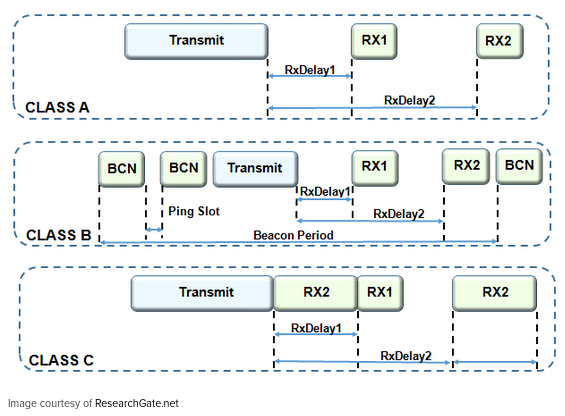
\includegraphics[width=0.7\textwidth]{img/endDevices.png}
			\caption{Funcionamiento de nodos finales usando LoRaWAN.}
		\end{center}
	\end{figure}
	
	\pagebreak
	
	\noindent \textbf{Estructura de un paquete LoRaWAN}
	
	\begin{figure}[h]
	\begin{center}
			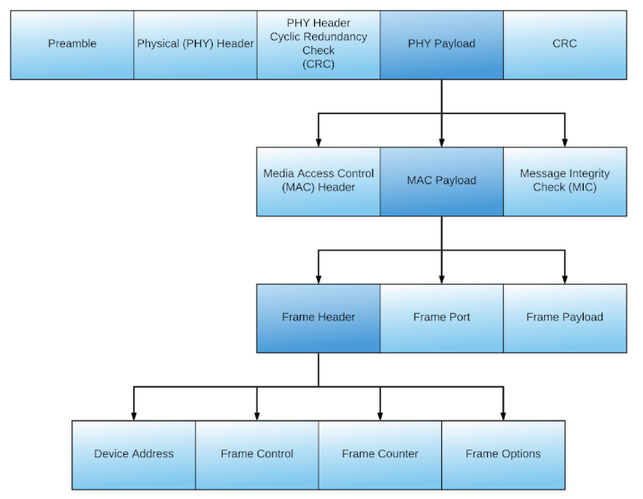
\includegraphics[width=0.7\textwidth]{img/lora_phyLayer_packetFormat.png}
			\caption{Estructura general de un paquete LoRaWAN.}
	\end{center}
	\end{figure}
	

	
	\begin{figure}[h]
	\begin{center}
			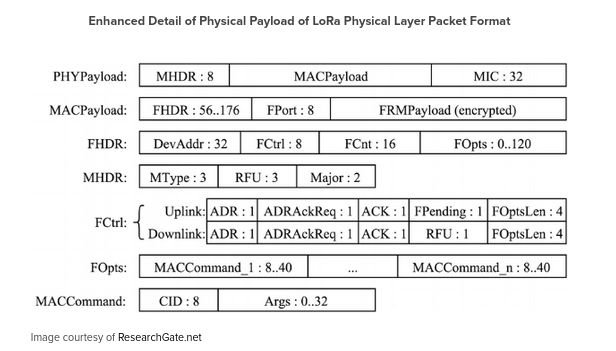
\includegraphics[width=0.7\textwidth]{img/lora_phyLayer_packetFormat_enh.png}
			\caption{Estructura detallada de un paquete LoRaWAN.}
	\end{center}
	\end{figure}

	\pagebreak

	\subsection[Monitorización y automatización]{Monitorización y automatización}
	
	El Arduino que vamos a usar es el Arduino nano, como ya se ha comentado anteriormente. Los sensores que vamos a usar son:
	
	\pagebreak
	\subsection[Comunicaciones LoRa]{Comunicaciones LoRa}
	%Simulaciones Xirio? O mejor abajo? + calculo teorico de perdidas en el enlace/balance de enlace
	Los módulos LoRa que vamos a usar son los E32-868T30D (como ya se ha comentado anteriormente).
	\subsubsection{Cálculo teórico de pérdidas de enlace}
	\subsubsection{Simulación en \textit{Radio Mobile}}
	
	\subsection[Resumen del capítulo]{Resumen de capítulo}
	
	En este capítulo se ha hablado de las dos principales tecnologías usadas en este proyecto. Se han explicado de forma teórica, después se ha explicado cómo se integran en el proyecto en la parte de monitorización y automatización en el caso de Arduino, y en la parte radio en el caso de LoRa. Se hace un acercamiento a software de simulación radio. Se sacan conclusiones para la creación de un prototipo que pueda ser ejecutado y probado en el entorno objetivo.
	\pagebreak
	
	
	\section[Prototipo y pruebas]{Prototipo y pruebas}
	
	% Ensamblado PCB y pruebas
	\subsection[Ubicación]{Ubicación}
	\subsection[Prototipo inicial]{Prototipo inicial}
	\subsection[Prototipo definitivo]{Prototipo definitivo}
	\subsection[Pruebas]{Pruebas}
	\subsection[Comentarios sobre los resultados de las pruebas]{Comentarios sobre los resultados de las pruebas}
	\subsection[Presupuesto]{Presupuesto}
	\subsection[Resumen del capítulo]{Resumen del capítulo}
	
	\section[Conclusiones y líneas futuras]{Conclusiones y líneas futuras}
	
	\section*{Glosario}
	\addcontentsline{toc}{section}{Glosario}
	
	\section*{Bibliografía}
	\addcontentsline{toc}{section}{Bibliografía}
	
	\section*{Anexos}
	\addcontentsline{toc}{section}{Anexos}
	
	\subsection*{Anexo I}
	\addcontentsline{toc}{subsection}{Anexo I}	
	
	\subsection*{Anexo II}
	\addcontentsline{toc}{subsection}{Anexo II}
	
\end{document}